\documentclass[a4paper,11pt]{article}
\usepackage[margin=22mm,headheight=16pt,footskip=10mm]{geometry}
\usepackage{fontspec}
\setmainfont{Times New Roman}
\setsansfont{Arial}
\setmonofont{Consolas}[Scale=.87]
\usepackage{amsmath,amssymb,amsthm,graphicx,booktabs,tabularx,longtable,array}
\usepackage{setspace,titlesec,fancyhdr,caption,enumitem,needspace,placeins,float}
\usepackage[hidelinks,unicode,bookmarksnumbered]{hyperref}
\usepackage{xurl}
\setstretch{1.22}
\setlength{\parindent}{1.5em}
\setlength{\parskip}{3pt}
\setlength{\emergencystretch}{2em}
\clubpenalty=10000
\widowpenalty=10000
\renewcommand{\arraystretch}{1.13}
\setlength{\tabcolsep}{4.5pt}
\titleformat{\section}{\Large\sffamily\bfseries}{\thesection}{.7em}{}
\titleformat{\subsection}{\large\sffamily\bfseries}{\thesubsection}{.7em}{}
\titlespacing*{\section}{0pt}{15pt}{7pt}
\titlespacing*{\subsection}{0pt}{10pt}{5pt}
\pagestyle{fancy}
\fancyhf{}
\fancyhead[L]{\small Event-day metro demand and timetable adjustment}
\fancyhead[R]{\small Research manuscript}
\fancyfoot[C]{\thepage}
\renewcommand{\headrulewidth}{.3pt}
\newtheorem{theorem}{Theorem}[section]
\newtheorem{proposition}[theorem]{Proposition}
\newtheorem{lemma}[theorem]{Lemma}
\numberwithin{equation}{section}
\captionsetup{font=small,labelfont=bf}
\newcommand{\R}{\mathbb R}
\newcommand{\E}{\mathbb E}
\newcommand{\argmin}{\operatorname*{arg\,min}}
\newcommand{\ind}{\mathbf 1}
\hypersetup{pdftitle={Event-Day Metro Demand Forecasting and Timetable Adjustment: A Retrospective Dadaocheng Study},
 pdfauthor={Statistical Practice Research Group},
 pdfsubject={Forecast benchmarks, queueing simulation, timetable search, proofs, and empirical limitations}}
\begin{document}
\begin{center}
{\LARGE\sffamily\bfseries Event-Day Metro Demand Forecasting\\and Timetable Adjustment}\\[6pt]
{\large\sffamily\bfseries A Retrospective Study of Dadaocheng Fireworks Events}\\[8pt]
Statistical Practice Research Group\\
Research manuscript, 19 November 2026
\end{center}
\vspace{4pt}
\noindent\textbf{Abstract.}
We study a linked planning problem for special-event rail service: forecast station-level hourly entries before an event, examine plausible within-hour arrival patterns, and compare Green-line timetables under capacity and waiting assumptions. The event panel contains 21 events, four stations and six evening hours per event (504 station-hour observations). Nine Beimen events in 2024--2026 (54 hours) are evaluated by forward-year splits. Three newly computed, past-only forecasting benchmarks are compared on exactly these folds: an ordinary-day profile, a prior-year event median, and an ordinary-day profile plus a historical event excess. Their Beimen mean absolute errors (MAEs) are 2,027.50, 1,339.26 and 1,233.76 entries per hour, respectively; the archived weighted XGBoost model obtains 440.28. However, the nine events were repeatedly inspected during earlier model development, and historical source-publication times are not fully certified, so these are retrospective comparisons, not an unbiased prospective deployment test. Minute-level queueing is evaluated under assumed uniform, broad-peak and concentrated-peak arrivals. A later full-line simulation compares the reference Green-line timetable with candidate add, cancel and retime plans over 18:00--23:00. At the illustrative waiting-value multiplier of one, an eight-event independent-scenario evaluation finds a decrease in mean waiting from 3.895 to 2.868 minutes, together with 496 added and zero cancelled services and an increase of TWD 2.384 million in modeled variable operating expenditure. We derive the relevant penalized-estimation and finite-horizon queue identities, prove existence only for the stated estimation and finite-candidate problems, and identify data and operating constraints that prevent interpretation as a field-ready dispatch instruction.

\noindent\textbf{Keywords:} special-event ridership; forward validation; simple benchmarks; XGBoost; batch-service queue; metro timetable; cost--waiting trade-off.
\vspace{7pt}
\tableofcontents
\clearpage
\pagenumbering{arabic}

\section{Introduction}
\subsection{Research problem}
Fireworks dispersal may concentrate thousands of passengers within a short time at Beimen and nearby stations. For operations planning, three distinct quantities must not be conflated: hourly tap-in demand, the minute at which a passenger reaches a platform, and the available space on a passing train. A plausible hourly forecast can still yield an inadequate timetable when its largest hour is underpredicted or when arrivals cluster within that hour. Conversely, a timetable that reduces simulated waiting may incur additional cash expenditure. This study therefore follows the complete chain from data to an explicitly limited timetable decision.

The research questions are:
\begin{enumerate}[leftmargin=2em]
\item How well does the frozen event-day hourly forecast perform relative to transparent rules that use the same chronological cutoffs and evaluation events?
\item How sensitive is platform waiting to unobserved within-hour arrivals and train space?
\item Relative to a reference timetable, what operating-expenditure and waiting-time trade-offs arise when Green-line services may be added, cancelled or retimed?
\end{enumerate}
The first two questions are statistical and simulation questions; the third is a finite-candidate decision comparison. The paper makes no causal claim that a particular festival attribute independently creates a stated number of metro entries, and it does not infer a real-time train-dispatch order.

\subsection{Study contributions and scope}
The contribution is a reproducible, auditable sequence rather than a new forecasting algorithm. First, all models and three simple benchmarks share forward-year test folds. Second, the information available at the proposed day-before forecast time is separated from retrospective measurements. Third, hourly predictions feed explicit minute-arrival and capacity scenarios rather than an unlabelled queueing calculation. Fourth, the latest timetable experiment keeps the original Green-line service as a comparator and reports cash expenditure separately from monetized waiting. A companion appendix states mathematical results and their assumptions. Figure~\ref{fig:workflow} summarizes the sequence; its editable source is \texttt{workflow\_en.mmd}.
\begin{figure}[htbp]\centering
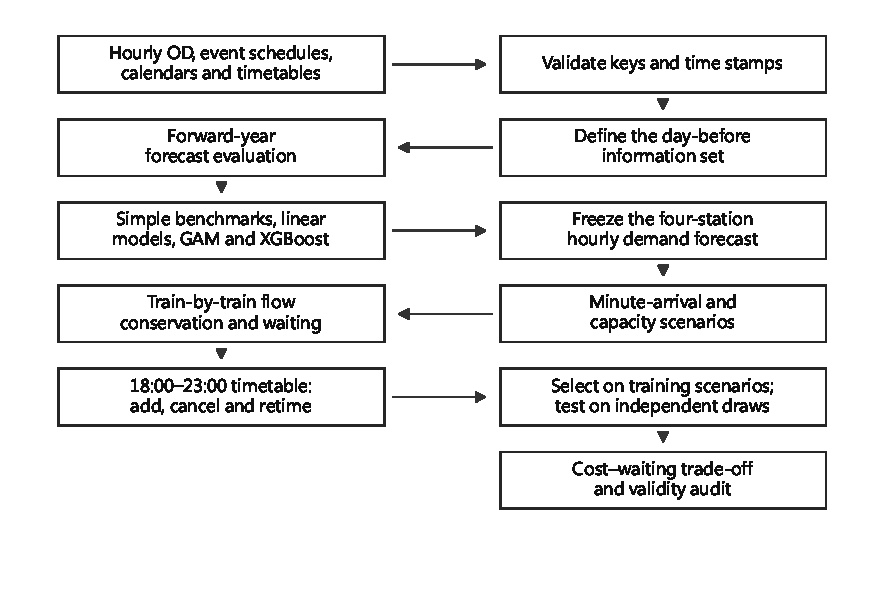
\includegraphics[width=.94\linewidth]{workflow_en.pdf}
\caption{Research workflow. Boxes distinguish forecasting, conditional queue simulation, and timetable evaluation. The diagram is a design description, not evidence that every input is prospectively available.}
\label{fig:workflow}
\end{figure}

\section{Related literature and methodological rationale}
Ridge regression shrinks coefficients when regressors are strongly correlated, while the Lasso can set coefficients to zero \cite{ridge,lasso}. These properties justify including both as interpretable linear comparators; they do not imply that either must predict event peaks well. Generalized additive models (GAMs) offer smooth nonlinear partial effects while retaining additive interpretability \cite{gam,pspline}. XGBoost can represent threshold and interaction patterns with regularized boosted trees \cite{xgb}. We therefore compare model families with distinct inductive biases, rather than claiming that more complex models are intrinsically preferable.

Temporal evaluation must preserve chronology and event grouping. Forward-origin validation motivates the annual splits \cite{fpp}. Nevertheless, repeated inspection of the same small set of final events can produce selection bias even if individual fitting steps are chronologically correct \cite{cawley}. This distinction matters here because the fourfold dispersal training weight was retained after comparisons involving the nine events.

For waiting, Little's steady-state relation is informative but not a license to treat a fireworks surge as a stationary M/M/$c$ queue \cite{little}. We use a finite-horizon, train-arrival batch-service representation and derive its passenger-minute accounting directly. Rail-corridor research has considered passenger waiting and operating cost jointly \cite{pan}; our cost function and candidate search are specific to this project and are not presented as a reproduction of that paper's model. These references support the methodological families, while the numerical settings below remain project assumptions.

\section{Data and study design}
\subsection{Observation units and provenance}
The outcome is the number of tap-ins at station $s$ during source hour $h$ on held event date $d$, denoted $Y_{dsh}$. The four stations are Beimen, Daqiaotou, Shuanglian and Minquan West Road; the hours are 18:00--23:00. Twenty-one events yield $21\times4\times6=504$ rows. Rows from one event share many determinants and are not 504 independent events. The main forecast evaluation is the nine Beimen events from 2024, 2025 and 2026, hence $9\times6=54$ rows.

The primary source is Taipei Metro's hourly origin--destination (OD) data \cite{metrodata}. In the source convention, an OD record associated with a destination such as Beimen retains its \emph{origin} time bin; aggregating such records by destination is not a direct hourly exit-gate count. Published calendars and pre-announced event programs supply candidate date and dispersal features. Official timetable PDFs and adjacent-station travel times supply an operational reference, but the available timetable edition is not confirmed to be the actual historical timetable of every event. Observed weather from the Central Weather Administration, annual budget records, social posts and search interest provide contextual or exploratory information; observed weather and annual expenditure are not inserted into the frozen day-before demand model.

\begin{table}[htbp]\centering\small
\caption{Data layers, units, and their analytical roles.}
\label{tab:data}
\begin{tabularx}{\linewidth}{p{32mm}p{42mm}X}\toprule
Layer & Native unit & Role and qualification\\\midrule
Metro OD & origin station, destination station, source hour & Hourly outcome and background flow; historical release dates remain incompletely audited.\\
Event and calendar & event date, announced program, weekday/holiday & Scheduled dispersal overlap and date descriptors; actual ending time is excluded from the day-before model.\\
Ordinary-day reference & station, source hour, selected comparator dates & Retrospective 56-day station-hour baseline; both a model feature and a standalone rule in this paper.\\
Train timetable & service, direction, station, time & Reference and candidate service schedules; not a certified record of every historical event-day dispatch.\\
Train loading & inferred passengers per service & Simulated from OD and routing; matched historical measured train loads are unavailable.\\
Weather, publicity, finance & observation time, post, or fiscal year & Contextual/sensitivity information; an annual publicity total is not a per-event amount.\\\bottomrule
\end{tabularx}
\end{table}

\subsection{The ordinary-day reference and the information frontier}
The archived feature \texttt{retrospective\_baseline\_56d}, here written $B_{dsh}$, averages at most four nearest eligible comparator days selected among the preceding eight same weekdays. Selection excludes listed event days and incomplete 18:00--24:00 records and requires matching holiday/makeup-workday classification and calendar note; at least two days are required for the original event-level eligibility rule. It is \emph{not} an average over every day in a 56-day block. An independent hourly replay stored at \texttt{.local/research\_review/2026-10-07-independent-review/independent\_hourly\_baselines.csv} reproduces all 504 archived baseline values to numerical tolerance (maximum absolute difference $2.84\times10^{-14}$). This reconciles the calculation, not the historical public availability of each input. The earlier four-week/eight-week event-versus-normal analysis is a separate descriptive comparison, not a forecasting score on the same nine-event panel.

Let $t_0(d)$ be the planned forecast issue time on the day before event $d$. A true prospective input requires
\begin{equation}
\operatorname{available\_at}(X_{dsh,j})\leq t_0(d)
\quad\text{for every input column }j.
\label{eq:frontier}
\end{equation}
Calendar fields can be computed before $d$; scheduled ending times can be used only if their announcement preceded $t_0(d)$. Actual event end times, observed weather and post-event social volume do not meet this rule. The annual holdout experiments follow a day-before \emph{design}, but the release timestamps of all historical OD and calendar snapshots were not fully reconstructed. Thus the work is a retrospective as-of sensitivity study, not a verified deployable D$-1$ forecast.

\subsection{Data processing, missingness, and storage}
The analysis key is $(d,s,h)$. Numeric parsing, duplicate checks, six-hour coverage checks and station labels precede estimation. Optional fields have missingness indicators and training-fold-only imputation; missing is not silently recoded to observed zero. Continuous features are standardized using training-fold moments, and categories and interaction columns are learned from that fold. Exact linear dependencies are removed without consulting outcomes. The OD preparation uses DuckDB and Parquet for large scans; relational MySQL tables store activities, weather observations, station metadata and annual finance with keys. This storage division affects reproducibility and query cost but not the statistical estimand. Raw/private snapshots and model artifacts are excluded from the public repository, so the manuscript gives both source identifiers and a private-input reproduction requirement.

\section{Forecasting methods}
\subsection{Comparable simple benchmarks}
Let $\mathcal T_y$ contain only events in years strictly before test year $y$. For each held-out $(d,s,h)$ with $d$ in year $y$, we evaluate three rules without fitting a flexible predictor:
\begin{align}
\widehat Y^{(B)}_{dsh}&=B_{dsh}, \label{eq:baseordinary}\\
\widehat Y^{(E)}_{dsh}&=\operatorname{med}_{e\in\mathcal T_y}Y_{esh}, \label{eq:baseevent}\\
\widehat Y^{(B+E)}_{dsh}&=
\left[B_{dsh}+\operatorname{med}_{e\in\mathcal T_y}
  (Y_{esh}-B_{esh})\right]_+ . \label{eq:baseincrement}
\end{align}
The historical-event median is conditional on the same station and source hour; the excess rule transfers a prior-year median event increment to the current ordinary-day level. All predictions are clipped at zero. The first two rules are already nonnegative. No labels from the held-out year enter either median, and all three rules are scored on the same nine Beimen events as the frozen models. In contrast, $B_{dsh}$ can use earlier ordinary days from the target year because the archived feature was defined relative to each event date. Its contemporaneous release status remains unverified. These rules do not contain a forecasted event size, and the two event-analog rules are intentionally simple rather than tuned on the nine held-out events.

\subsection{Candidate features and common evaluation}
The model candidate set comprises station and source hour, their interaction, weekend status, day of year, a year trend, the ordinary-day level, and the first and second hours of overlap after a \emph{scheduled} finale, by station. Planned drone or weather variables were explored separately but are not part of the retained model. Standardized continuous columns are transformed using training-only moments; category references, imputation values and any rank-based column removal are also estimated inside the training fold. Strong correlation or a large variance-inflation factor warns about coefficient instability, but is neither a proof of causality nor an automatic instruction to remove a predictor from every model.

For test year $y\in\{2024,2025,2026\}$, fit on all preceding events and evaluate the complete Beimen events in year $y$. The training sets contain 12, 15 and 18 events, respectively. All six hours of an event stay together. Hyperparameter comparison within a year uses only earlier years; nevertheless, subsequent decisions made after examining these nine outer events introduce an additional model-selection risk. Define the primary forecast error and two peak-related summaries by
\begin{align}
\operatorname{MAE}&=\frac1n\sum_i|Y_i-\widehat Y_i|,&
\operatorname{RMSE}&=\sqrt{\frac1n\sum_i(Y_i-\widehat Y_i)^2},\label{eq:metrics}\\
\operatorname{Under}_{\mathcal D}
&=\sum_{i\in\mathcal D}a_i(Y_i-\widehat Y_i)_+,&
\operatorname{PeakAbs}
&=\frac1{|\mathcal E|}\sum_{e\in\mathcal E}
  |Y_{e,h_e^*}-\widehat Y_{e,h_e^*}|.\label{eq:peakmetrics}
\end{align}
Here $h_e^*=\arg\max_hY_{eh}$ is the \emph{observed} peak hour, used for retrospective scoring only. $\mathcal D$ and weights $a_i$ are determined from scheduled dispersal-hour overlap, normalized within events and then equally across events; if no scheduled overlap is known, the six event hours receive fallback weight. MAE and RMSE are per source hour. Positive underprediction and absolute peak error address different operational concerns.

\subsection{Linear models, GAM and tree boosting}
For treatment-coded and standardized design matrix $Z$ and training response $Y$, ordinary least squares minimizes $\|Y-\beta_0\mathbf1-Z\beta\|^2$. Ridge adds a squared penalty,
\begin{equation}
\min_{\beta_0,\beta}\,
\frac1n\|Y-\beta_0\mathbf1-Z\beta\|_2^2+
\lambda_R\|\beta\|_2^2,\qquad \lambda_R>0.
\label{eq:ridge}
\end{equation}
The Lasso replaces the penalty by $\lambda_L\|\beta\|_1$ \cite{lasso}. Ridge keeps correlated signals but shrinks them; Lasso can remove individual encoded columns and hence is more sensitive to scaling and penalization when predictors are related. These are conditional predictive associations, not treatment effects.

The Gaussian-identity GAM uses an additive linear predictor
\begin{equation}
g(X)=\beta_0+\sum_{j\in\mathcal S}f_j(X_j)+
\sum_{k\in\mathcal L}\theta_kX_k ,
\label{eq:gam}
\end{equation}
with cubic P-splines for approved smooth terms, second differences of spline coefficients penalized, and a positive all-coefficient $L_2$ term for stability \cite{gam,pspline}. The ordinary-day baseline is linear in this implementation. A partial-effect curve describes one component of this fitted additive function; its horizontal position is not a forecast error or a causal date effect.

XGBoost adds regularized trees $f_m$ sequentially \cite{xgb}. For a fixed candidate tree structure and a leaf with summed first and second derivatives $G_j,H_j$, the quadratic approximation has optimal leaf weight
\begin{equation}
w_j^*=-\frac{G_j}{H_j+\lambda_T},\qquad H_j+\lambda_T>0.
\label{eq:leaf}
\end{equation}
This is an optimum \emph{conditional on that leaf and approximation}; it proves neither a globally optimal tree ensemble nor superior external accuracy. Trees are included because threshold patterns and multiway station--hour--dispersal interactions need not be specified one at a time.

\subsection{Tuning, training weights and deployment choice}
The archived experiments inspected 25 Ridge penalties, 60 GAM smoothness/coefficient-penalty/basis combinations, and 180 prespecified XGBoost configurations (not the complete Cartesian product). Learning-rate/tree-count pairs and early stopping were also examined. After adding the ordinary-day feature, a previously fixed tree setting outperformed some retuned alternatives. The retained version uses the original year-specific tree settings and a training weight for Beimen scheduled dispersal:
\begin{equation}
\widetilde\omega_i=
1+3\,\ind\{s_i=\mathrm{Beimen}\}(o_{i,0\text{--}60}+o_{i,60\text{--}120}),
\qquad
\omega_i=\frac{\widetilde\omega_i}
{\overline{\widetilde\omega}_{\,e(i)}}.
\label{eq:weights}
\end{equation}
The denominator is the mean raw weight within the corresponding event. This fourfold maximum \emph{training-sample} emphasis is distinct from an asymmetric loss that charges twice as much for underprediction, and distinct from weights in a model fusion. The final model has depth 3, 250 trees and learning rate 0.10 in the 2024 fold; depth 4, 250 trees and learning rate 0.05 in the 2025 and 2026 folds. The retained settings use minimum child weight 1, $L_2$ leaf penalty 1, no $L_1$ leaf penalty and full row/column sampling; the final fit does not use early stopping.

Equal-weight and learned nonnegative combinations of Ridge, GAM and XGBoost were compared. Neither consistently surpassed the best tree in the archived comparison; the deployed demand input is therefore the single frozen weighted XGBoost, while linear models and GAM remain explanatory comparators. The existence of a minimum for a fusion-weight loss does not guarantee useful out-of-sample complementarity. Mathematical conditions are given in Appendix~\ref{sec:proofs}.

\section{Forecasting results}
\subsection{Simple baselines on identical held-out events}
Table~\ref{tab:benchmarks} reports the new standalone baselines and the archived forecast, evaluated using precisely the nine Beimen events and scorer in Section 4.2. The best simple rule is the ordinary-day level plus a prior-year station-hour median event excess. Its MAE of 1,233.76 is substantially smaller than the ordinary-day-only MAE of 2,027.50, demonstrating why the normal-day level is a weak \emph{sole} forecast for a special event. The frozen weighted XGBoost's MAE of 440.28 is lower by 793.48 entries per hour relative to that strongest simple rule. This is a retrospective comparison, not a claim of unbiased future improvement.
\begin{table}[htbp]\centering\small
\caption{Same-fold Beimen forecast comparison: nine events, 54 hours; counts are entries per hour.}
\label{tab:benchmarks}
\begin{tabular}{p{50mm}rrrr}\toprule
Method & MAE & RMSE & Peak absolute & Dispersal under\\\midrule
Ordinary-day profile & 2,027.50 & 3,281.47 & 6,277.41 & 4,628.28\\
Prior-year event median & 1,339.26 & 2,043.67 & 3,269.56 & 2,450.87\\
Ordinary + prior-year median excess & 1,233.76 & 1,940.49 & 3,196.39 & 2,320.54\\
\textbf{Frozen weighted XGBoost} & \textbf{440.28} & \textbf{690.91} & \textbf{747.14} & \textbf{483.61}\\\bottomrule
\end{tabular}
\end{table}
\begin{figure}[htbp]\centering
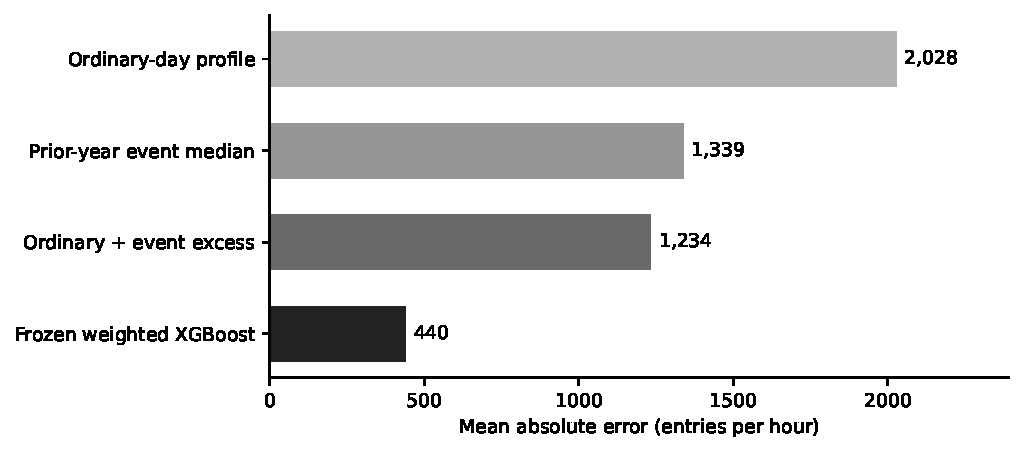
\includegraphics[width=.91\linewidth]{../../result/research_paper/figures/forecast_benchmark.pdf}
\caption{Hourly MAE for three prespecified simple rules and the archived weighted XGBoost on the same nine Beimen events. Lower is better.}
\label{fig:benchmark}
\end{figure}

\begin{table}[htbp]\centering\small
\caption{Event-level MAE for the strongest simple rule and frozen weighted XGBoost.}
\label{tab:eventmae}
\begin{tabular}{lrr@{\qquad}lrr}\toprule
Event & Excess rule & XGBoost & Event & Excess rule & XGBoost\\\midrule
2024-07-17 & 939.6 & 260.6 & 2025-08-20 & 782.4 & 220.3\\
2024-07-31 & 1,071.4 & 338.4 & 2025-08-30 & 1,861.2 & 326.8\\
2024-08-10 & 2,294.9 & 1,384.7 & 2026-07-25 & 1,312.5 & 375.5\\
2025-08-06 & 730.2 & 232.5 & 2026-08-05 & 487.3 & 275.5\\
2026-08-15 & 1,624.5 & 548.2 & & &\\\bottomrule
\end{tabular}
\end{table}
The XGBoost MAE is smaller on each of these nine events, but the worst event still has MAE 1,384.7. A paired resampling of \emph{events} yields a descriptive 2.5--97.5 percentile range of 566--1,035 entries per hour for the MAE advantage over the excess rule (20,000 fixed-seed resamples). It is not a confidence interval with guaranteed coverage for future events: only nine events are available, years may be dependent, and the frozen model itself was selected with prior inspection of this cohort. No statistical significance claim is based on this interval.

\subsection{Archived model-family comparisons and peak limitation}
On the same nine Beimen events, the archived Ridge, GAM, unweighted tree and weighted tree results are as in Table~\ref{tab:modelcompare}. This table answers a different question from Table~\ref{tab:benchmarks}: whether added model structure helped \emph{among the already constructed models}. The fourfold dispersal weight reduces MAE by about 7.1\% relative to the unweighted XGBoost, yet the scheduled dispersal-window underprediction increases from 405.96 to 483.61. The average-error improvement cannot be substituted for a claim that platform overload risk is resolved.
\begin{table}[htbp]\centering\small
\caption{Archived model-family results on the same nine-event Beimen cohort.}
\label{tab:modelcompare}
\begin{tabular}{lrrrr}\toprule
Model & MAE & RMSE & Peak absolute & Dispersal under\\\midrule
Ridge & 845.44 & 1,547.49 & 2,681.26 & 1,413.98\\
GAM & 830.71 & 1,315.75 & 2,305.11 & 1,132.68\\
XGBoost, unweighted & 473.91 & 766.90 & 749.02 & 405.96\\
XGBoost, dispersal weighted & 440.28 & 690.91 & 747.14 & 483.61\\\bottomrule
\end{tabular}
\end{table}

The teammate's separate linear sensitivity experiment retuned a different Ridge path and obtained original-scaling MAEs of 846.33 (OLS), 851.20 (retuned Ridge) and 848.52 (Lasso). Its Lasso improvement over that \emph{retuned} Ridge is only 2.68 entries per hour; the treatment of encoded columns and tuning differs from the frozen Ridge line above. The lower ex-post minimum along an inspected Lasso penalty path is not a selected prospective result. Thus Lasso remains a useful sparsity sensitivity analysis, but does not replace the retained forecast.

Figure~\ref{fig:peak} shows 10 August 2024. The observed Beimen maximum is about 11,101 entries, while the weighted tree predicts about 8,359 at that observed peak hour, an underprediction of about 2,742 (24.7\%). A station-hour ordinary-day profile is much lower. The event illustrates why a dispatch simulation should vary both demand error and remaining train capacity even if overall MAE is modest.
\begin{figure}[htbp]\centering
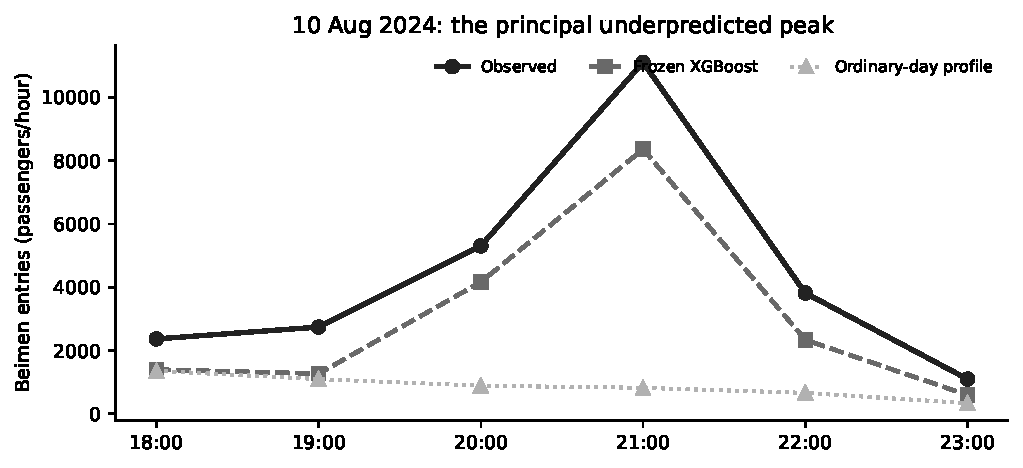
\includegraphics[width=.92\linewidth]{../../result/research_paper/figures/peak_profile.pdf}
\caption{Observed and predicted Beimen entries on 10 August 2024. The ordinary-day curve is a retrospective baseline, not an observed event-day forecast issued at the time.}
\label{fig:peak}
\end{figure}
\FloatBarrier

\section{From hourly demand to finite-horizon waiting}
\subsection{Unobserved minute arrivals as explicit scenarios}
Hourly tap-ins do not reveal the minute at which a passenger reaches a platform. For a predicted total $\widehat N_{dsh}$, let $p_{dshm}\geq0$ be the fraction allocated to minute $m\in\{0,\ldots,59\}$, with $\sum_mp_{dshm}=1$. The implied minute mass is
\begin{equation}
A_{dshm}=\widehat N_{dsh}p_{dshm}.
\label{eq:minute}
\end{equation}
The first Beimen experiment compares uniform allocation with truncated broad and concentrated peaks (standard deviations 20 and 5 minutes), alternative peak centers at minute 15, 30 or 45, and directional splits near 40:60, 50:50 and 60:40. Only the model-predicted highest hour receives a nonuniform shape in this early experiment; other hours remain uniform. This is a sensitivity design, \emph{not} an estimate that actual fireworks passengers follow a Gaussian minute profile. A five-minute access-to-platform delay is an assumption rather than a measured distribution.

\subsection{Batch-service queue and passenger-minute identity}
Let $Q_{j-1}$ be passengers left after train $j-1$, $A_j$ new arrivals before train $j$, and $C_j$ the space available to this queue on train $j$. With alighting before boarding, the fluid-count recurrence is
\begin{equation}
Q_j^-=Q_{j-1}+A_j,\qquad
B_j=\min(Q_j^-,C_j),\qquad
Q_j=Q_j^--B_j.
\label{eq:queue}
\end{equation}
This nonnegative conservation law is a train-arrival batch service, not a continuous-service stationary M/M/$c$ queue. If a passenger $\ell$ arrives at minute $a_\ell$ and boards at minute $b_\ell$, while an unserved passenger has $b_\ell>T$, then the total waiting inside horizon $[0,T]$ is
\begin{equation}
W_T=\int_0^T Q(t)\,dt
=\sum_\ell[\min(b_\ell,T)-a_\ell]_+ .
\label{eq:area}
\end{equation}
The equality follows by writing $Q(t)=\sum_\ell \ind\{a_\ell\leq t<\min(b_\ell,T)\}$ and interchanging a finite sum with the integral. It counts only \emph{truncated} waiting for passengers still unserved at $T$. Extending the reference timetable to a common clearing horizon, or reporting residual queues, is necessary before comparing plans. Little's $L=\lambda W$ is a steady-state result \cite{little}; Equation~\eqref{eq:area} is the finite-horizon identity used here.

\subsection{Initial Beimen-only scenario results}
The first study evaluates 1,134 combinations from nine events under the then-current timetable. Remaining space is assumed to be 25\%, 50\% or 75\% of a six-car nominal maximum of 2,220 passengers, corresponding to 555, 1,110 and 1,665 spaces; these are \emph{not} observed carriage loads. Table~\ref{tab:queue} reports event-equal mean waiting after the relevant scenario queues clear. The concentrated peak with only 25\% assumed space produces 7.94 minutes, against 3.39 for a uniform arrival pattern under the same nominal hourly totals. This demonstrates sensitivity to shape and space, not evidence that one shape actually occurred.
\begin{table}[htbp]\centering\small
\caption{Initial Beimen scenario mean waits, minutes; nine events.}
\label{tab:queue}
\begin{tabular}{lrrr}\toprule
Within-hour arrival & 25\% remaining & 50\% remaining & 75\% remaining\\\midrule
Uniform & 3.39 & 3.12 & 3.12\\
Broad peak, SD 20 min & 4.10 & 3.12 & 3.12\\
Concentrated peak, SD 5 min & 7.94 & 4.22 & 3.52\\\bottomrule
\end{tabular}
\end{table}
\begin{figure}[htbp]\centering
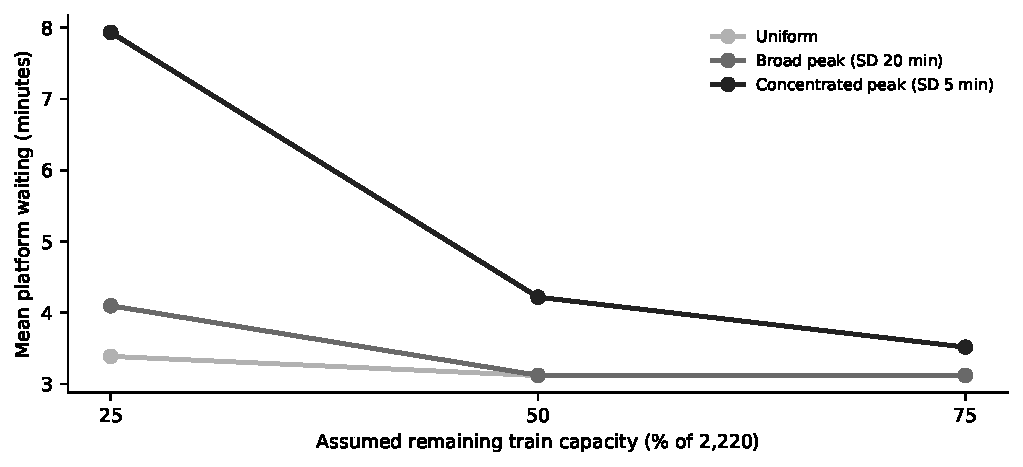
\includegraphics[width=.91\linewidth]{../../result/research_paper/figures/queue_shapes.pdf}
\caption{Conditional Beimen waiting by assumed minute-arrival concentration and remaining train capacity. This single-station experiment must not be numerically pooled with the later full-line model.}
\label{fig:queue}
\end{figure}
\FloatBarrier

\section{Full-line timetable evaluation}
\subsection{Reference schedule, passengers and service feasibility}
The later experiment takes an official Green-line timetable edition as its \emph{reference schedule} and permits add, cancel and retime operations for services whose Beimen departure falls in $[18{:}00,23{:}00)$. Trains outside that decision window and Red/Orange-line schedules are held fixed. Demand from 17:00--18:00 warms the network state; arrivals are injected until 23:00 and fixed later services continue clearing passengers to a common 02:00 terminal horizon. OD-derived trips are assigned by a shortest-time routing proxy; initial platform access and walking transfer time are assumed to be five minutes. Green-line train occupancy follows station-by-station boarding and alighting conservation with a six-car 2,220-person nominal bound. Connecting-line waiting can change when a passenger catches a different service, but full Red/Orange-line on-board capacities are not reconstructed.

Every altered or inserted service is checked against neighboring same-direction services, including those just outside the decision window. A 120-second minimum separation is a \emph{research constraint}, not a verified signaling-safety limit. An admissible solution also requires a finite, cleared waiting calculation in the specified model. Fleet availability, crew, depot departure, turnback, deadhead track conflicts and exact historical event-day train loads are not fully modeled. Thus passing these tests is weaker than being a physically executable operating order.

\subsection{Monetary objective and the meaning of a reference total}
For a candidate timetable $x$, let $N_+(x)$ and $N_-(x)$ be added and cancelled complete service trips after one-to-one matching of retimed trains. At the unverified variable-cost proxy of TWD 128.05 per train-kilometer, one 18.77-km full route plus one \emph{assumed} equal-length empty return for each added service, but only one avoided full-route service for a cancellation, gives
\begin{equation}
\Delta C_{\mathrm{op}}(x)=128.05(18.77)\{2N_+(x)-N_-(x)\}.
\label{eq:opcost}
\end{equation}
The matching prevents a retime from being counted as both a cancellation and an addition. Fixed payroll, depreciation and other unavoidable expenditures are not subtracted when a train is cancelled. The return movement is a cost assumption without separately modeled path capacity, and the train-kilometer proxy has not been verified against operator marginal-cost accounts.

Let $W_r(x)$ denote total passenger-minutes of waiting under training scenario $r$, and let $\gamma\in\{0.5,1,2\}$ represent a preference multiplier. The project uses the 2026 minimum hourly wage of TWD 196 \cite{wage} merely as an illustrative conversion, $v_0=196/60$ TWD per passenger-minute:
\begin{equation}
J_\gamma(x)=\Delta C_{\mathrm{op}}(x)
+\gamma\frac{196}{60}\frac1S\sum_{r=1}^{S}W_r(x),
\qquad x\in\mathcal P.
\label{eq:objective}
\end{equation}
The wage source supports the wage figure, \emph{not} an empirical claim that every passenger values waiting at that wage. $\gamma$ is not learned from operator choices, neural networks or inverse optimization. Monetary waiting is a welfare proxy rather than cash paid by the operator. Comparing operating expenditure separately from $W$ is therefore essential.

The project contains two quantities that could be described informally as a historical scheduling baseline. The older Beimen-oriented \emph{add-only} experiment stored a reference evaluation objective of about TWD 1.968 million over its eight events, under its own horizon, capacity and residual-queue assumptions. The current full Green-line add/cancel/retime experiment instead stores a reference timetable with 852 simulated services, operating proxy TWD 2.048 million and total waiting 6.425 million passenger-minutes over eight events. For $\gamma=1$, its \emph{modeled combined reference objective} is
\begin{equation}
J_1^{\mathrm{ref}}=
2{,}047{,}780.722+\frac{196}{60}(6{,}425{,}026.817)
=23{,}036{,}201.656\ \text{TWD}.
\label{eq:referenceobjective}
\end{equation}
This is the model value for the reference timetable, \emph{not} an observed historical dispatch bill or official net revenue. The older 1.968-million and current 23.036-million objectives have different passenger populations and conventions; they must not be differenced. All results below compare schedules only \emph{within} the current experiment.

\subsection{Candidate generation, selection and independent evaluation}
For each of eight assessable events, 200 simulated training scenarios are generated; the first 12 support proposal and initial screening. Candidate families include the earlier local search and a later 15-minute allocation grid. The 15-minute unit is a \emph{search bin}, not a train headway. The best training candidates from the earlier family remain available when the later family is added. For each $\gamma$, only training scenarios choose the timetable. A separate set of 300 draws evaluates the selected plan and the unaltered reference using paired inputs. These 500 draws are simulated alternatives, not 500 observed festivals. The earliest 2024 event is excluded from this eight-event dispatch test because no earlier comparable forecast-error event is available to construct its uncertainty scenarios.

The candidate set $\mathcal P$ is finite and contains the reference schedule. Therefore, if each candidate produces finite costs and waiting, the minimum of $J_\gamma$ over $\mathcal P$ exists. This is \emph{not} a proof that the heuristic generated all signaling-, fleet- and crew-feasible timetables, nor a proof of global operational optimality. The full statement and proof appear in Appendix~\ref{sec:proofs}.

\section{Timetable results and diagnostics}
\subsection{Eight-event comparison against the reference timetable}
At $\gamma=1$, Table~\ref{tab:dispatch} gives the independently evaluated, scenario-conditional comparison for the current full-line simulation. In total, 496 service trips are added, none are cancelled, and 608 are retimed according to the plan-matching rule. Mean waiting falls from 3.895 to 2.868 minutes (26.4\% fewer passenger-minutes), while modeled variable operating expenditure \emph{increases} by TWD 2,384,271. The selected plan's combined objective is TWD 19,885,398, lower than the reference value in Equation~\eqref{eq:referenceobjective} by TWD 3,150,803. This decrease is not a cash saving: operating expenditure rises, while monetized simulated waiting falls by more.
\begin{table}[htbp]\centering\small
\caption{Independent-scenario full-line comparison at $\gamma=1$. Cost changes are TWD relative to each reference timetable.}
\label{tab:dispatch}
\begin{tabular}{lrrr}\toprule
Event & Add/cancel/retime & Operating cost change & Mean wait: ref.\ $\to$ plan\\\midrule
2024-07-31 & 50/0/87 & +240,350 & 3.38 $\to$ 2.64\\
2024-08-10 & 78/0/65 & +374,946 & 4.67 $\to$ 3.23\\
2025-08-06 & 51/0/83 & +245,157 & 3.38 $\to$ 2.63\\
2025-08-20 & 58/0/88 & +278,806 & 3.38 $\to$ 2.59\\
2025-08-30 & 86/0/59 & +413,402 & 4.67 $\to$ 3.11\\
2026-07-25 & 56/0/68 & +269,192 & 4.64 $\to$ 3.35\\
2026-08-05 & 57/0/87 & +273,999 & 3.36 $\to$ 2.59\\
2026-08-15 & 60/0/71 & +288,420 & 4.64 $\to$ 3.31\\\midrule
Eight-event total/weighted mean & 496/0/608 & +2,384,271 & 3.89 $\to$ 2.87\\\bottomrule
\end{tabular}
\end{table}

The preference sensitivity in Table~\ref{tab:weightsensitivity} makes the operating--waiting trade-off explicit. Higher $\gamma$ increases the value assigned to saved waiting and hence selects more service in these candidates; it does not mean that the higher setting is empirically or ethically correct. The monetary objectives at different $\gamma$ values are not on a common preference scale and should not be ranked to estimate $\gamma$.
\begin{table}[htbp]\centering\small
\caption{Eight-event sensitivity to the illustrative waiting-value multiplier.}
\label{tab:weightsensitivity}
\begin{tabular}{rrrrr}\toprule
$\gamma$ & Added & Cancelled & Operating change (TWD) & Mean wait (min)\\\midrule
0.5 & 169 & 0 & +812,382 & 3.308\\
1.0 & 496 & 0 & +2,384,271 & 2.868\\
2.0 & 1,069 & 0 & +5,138,680 & 2.527\\\bottomrule
\end{tabular}
\end{table}
\begin{figure}[htbp]\centering
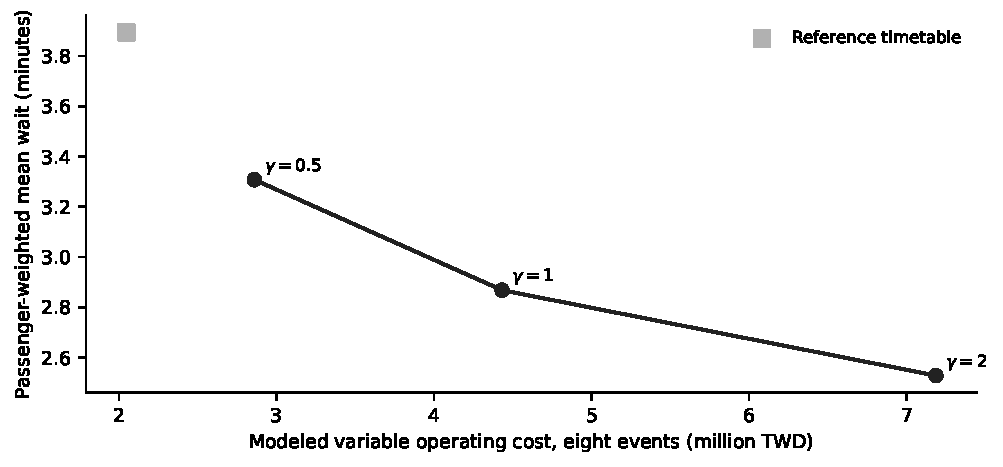
\includegraphics[width=.90\linewidth]{../../result/research_paper/figures/dispatch_tradeoff.pdf}
\caption{Modeled operating expenditure and waiting for the reference timetable and three selected preference scenarios. These are finite candidates, not a complete Pareto frontier.}
\label{fig:tradeoff}
\end{figure}

\subsection{Why cancellation was not selected}
A follow-up decomposition uses the \emph{same} eight-event, $\gamma=1$ selected plans and evaluation draws. Of the 1,694,410 passenger-minutes of modeled waiting reduction, 234,087 (13.8\%) belong to Beimen-classified journeys, 59,699 (3.5\%) to the other three study-station classes, and 1,400,624 (82.7\%) to other modeled passengers on the line. These are mutually assigned model groups, not measured counts of real passenger preferences. The large background group can make additional trains attractive in an all-passenger objective even if a Beimen-only criterion would choose differently. Early screening may also favor dense service; the decomposition is a diagnostic, not a proof that cancellation is never optimal.
\begin{figure}[htbp]\centering
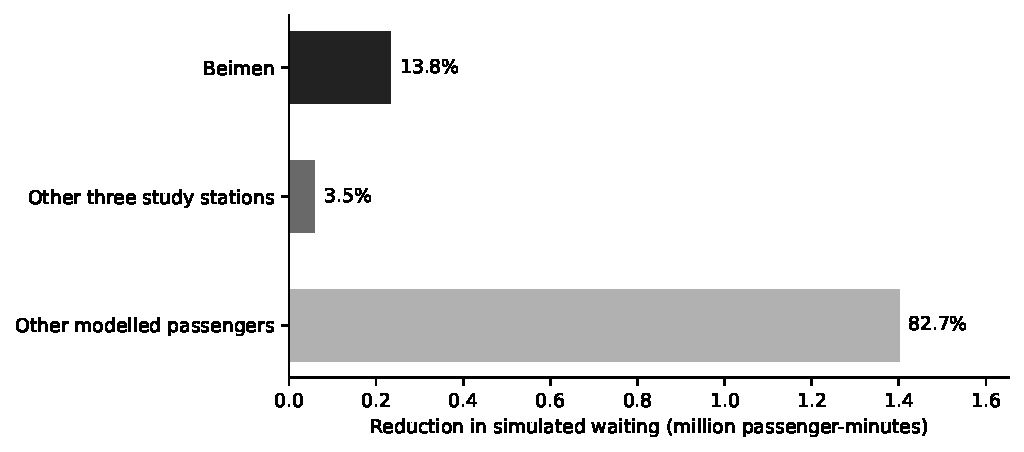
\includegraphics[width=.90\linewidth]{../../result/research_paper/figures/benefit_split.pdf}
\caption{Source of simulated waiting reduction for the selected $\gamma=1$ timetable, eight events combined. The background group is model-generated.}
\label{fig:benefit}
\end{figure}
Equation~\eqref{eq:opcost} makes cancellation of one full-route service worth approximately $c_-=128.05(18.77)=2{,}403.50$ TWD before waiting is counted. If all other decisions are fixed, cancellation is favorable at $\gamma=1$ only when the resulting increase in total expected waiting is below $c_-/(196/60)=735.76$ passenger-minutes. Multiple simultaneous changes can interact, so this is a local, conditional break-even calculation. A negative 15-minute heatmap cell is not itself a cancelled trip: retiming a service across adjacent grid cells also creates a negative and a positive cell.
\FloatBarrier

\subsection{Unknown train loading and operational validity}
Train free space in the later simulation is propagated from OD-derived flows, timetables and assumed routes. This is a meaningful improvement over assuming that every passing train has exactly 50\% free space, but it is \emph{not} a calibration to measured eight-event vehicle loads. A crowding-level API is a potential data-access lead \cite{crowding}; categorical live levels do not reconstruct historical numeric loads for the studied trains. If available space is systematically overestimated, simulated queues and the demand for extra trains will be understated; underestimation can yield excessive additional service. The most consequential next empirical input is matched train occupancy and minute-level platform/gate arrivals, followed by actual historical service and dispatch records.

\section{Discussion}
\subsection{What the comparisons establish}
The new simple benchmarks answer an important omission in the earlier manuscript: a model should not only be compared with other fitted models, but also with rules that would be easy to deploy and inspect. On the shared nine-event cohort, the retained XGBoost predicts more accurately than each tested simple rule for hourly MAE, RMSE, observed-peak absolute error and scheduled-dispersal underprediction. The most serious peak underprediction nevertheless remains large enough to matter for supply planning. The benchmark study was prespecified after an initial paper review but conducted on an already inspected cohort; it improves transparency, not the independence of the validation sample.

The queue study does not observe minute arrivals. It demonstrates a conditional operational consequence of two plausible axes of uncertainty: arrival concentration and remaining spaces. Likewise, the full-line timetable results demonstrate that, \emph{within the simulator and its candidate set}, lower passenger waiting can be purchased with more service. The 26.4\% simulated waiting reduction comes with TWD 2.384 million greater variable operating expenditure, not with simultaneous cash savings. Any claim of cost effectiveness depends on the time-value conversion, the number of background passengers, the service-cost proxy, and actual train capacities.

\subsection{Statistical and operational limitations}
There are only 21 event dates and nine repeatedly examined final Beimen events; 54 hourly test rows are not 54 independent festivals. Event-level bootstrap intervals from nine events are descriptive and do not address dependence within year, model-selection bias, uncertain publication times or future festival mix. The original ordinary-day comparator can itself be noisy when only two to four days qualify. A formal prospective study must archive source release times and hold out new events before inspecting their outcomes.

Hourly OD does not reveal minute platform arrivals or actual transfer paths. The current 2026 timetable edition is applied to earlier demand as a counterfactual reference rather than a certified historical reconstruction. The 2,220-person capacity, two-minute altered-service gap, walking times, operating cost and empty-return distance are assumptions or proxies. Existing train occupancy is inferred from OD, not observed. Fleet, crew, depot, turnback and complete signaling constraints are unavailable. Consequently, minimizing Equation~\eqref{eq:objective} over the generated plans does not yield an implementation-ready control-room order.

\subsection{Research priorities}
The next data collection should target (i) event-day minute gate or platform counts, (ii) matched per-train loads or sufficiently granular crowding proxies, (iii) actual historical timetable changes and depot/turnback feasibility, and (iv) verified source-publication timestamps. A newly occurring event can then provide a truly untouched forecast test. With these measurements, the queue input distribution and capacity transition can be calibrated and supply choices compared in an operating simulator that represents fleet and crew. Only after the information and feasibility layers are reliable would it be justified to test rolling-horizon rescheduling or to infer an operator's preference weight from observed decisions.

\section{Conclusion}
This retrospective case study connects event-day rail-demand prediction, conditional minute-level queues and a limited cost--waiting timetable comparison. It adds three transparent, same-fold forecast benchmarks missing from the previous paper draft. Across nine already inspected Beimen events, the frozen weighted XGBoost has MAE 440.28 entries per hour, compared with 1,233.76 for the strongest simple event-excess rule, but it still underestimates the largest observed 2024 peak by approximately 2,742 entries. In the full-line eight-event simulation, the selected $\gamma=1$ schedules reduce average modeled waiting from 3.895 to 2.868 minutes while adding 496 services and increasing modeled variable operating expenditure by TWD 2.384 million. The modeled combined objective improves, but this is not observed historical savings. The principal remaining scientific work is prospective validation and measurement of within-hour demand, train loading and deployable operating constraints.

\appendix
\section{Mathematical results and scope}\label{sec:proofs}
\subsection{Ridge and penalized additive model existence}
\begin{theorem}[Ridge existence and uniqueness]
Suppose $\lambda_R>0$, $Z$ and $Y$ are finite, and the intercept is unpenalized. Equation~\eqref{eq:ridge} has a unique coefficient vector and intercept, even if the columns of $Z$ are linearly dependent.
\end{theorem}
\begin{proof}
Let $H=I-\mathbf1\mathbf1^\top/n$, $Z_c=HZ$, and $Y_c=HY$. Minimizing over the intercept gives $\beta_0=\bar Y-\bar Z^\top\beta$. The remaining Hessian is $2(Z_c^\top Z_c/n+\lambda_R I)$, and for any nonzero $u$,
\[
u^\top(Z_c^\top Z_c/n+\lambda_R I)u
=\|Z_cu\|^2/n+\lambda_R\|u\|^2>0.
\]
The objective is strictly convex and coercive. Its unique coefficient minimum is
$\widehat\beta=(Z_c^\top Z_c+n\lambda_R I)^{-1}Z_c^\top Y_c$, with the corresponding unique intercept.
\end{proof}

\begin{proposition}[Penalized GAM coefficients]
For fixed spline bases, let $B$ be the design matrix and $D$ a second-difference penalty matrix. On a parameterization with duplicate intercept directions removed, the objective $\|Y-B\theta\|^2+\lambda_s\|D\theta\|^2+\lambda_c\|\theta\|^2$ has a unique minimum whenever $\lambda_c>0$.
\end{proposition}
\begin{proof}
Its Hessian is $2(B^\top B+\lambda_sD^\top D+\lambda_c I)$. For nonzero $u$, its quadratic form equals $2(\|Bu\|^2+\lambda_s\|Du\|^2+\lambda_c\|u\|^2)>0$ for $\lambda_s\geq0$. Hence the objective is coercive and strictly convex. An unpenalized intercept can be separated by centering or a full-rank identifiability constraint.
\end{proof}

\begin{proposition}[Lasso existence, not guaranteed coefficient uniqueness]
For finite $Z,Y$ and $\lambda_L>0$, the Lasso objective with an unpenalized intercept attains a minimum, although correlated design columns may allow several minimizing coefficient vectors.
\end{proposition}
\begin{proof}
Eliminate the intercept by centering as above. The objective $\|Y_c-Z_c\beta\|^2/n+\lambda_L\|\beta\|_1$ is continuous and coercive in $\beta$ because the penalty tends to infinity as $\|\beta\|\to\infty$. A compact nonempty sublevel set therefore contains a minimum. Strict convexity need not hold.
\end{proof}

\subsection{Fusion-weight existence and scale}
Let $P\in\R^{n\times3}$ contain out-of-fold base-model predictions, and consider squared-error weights. On the nonnegative simplex $\mathcal S_c=\{w\geq0:\mathbf1^\top w=c\}$ for any fixed $c>0$, the continuous loss $\|Y-Pw\|^2$ attains a minimum by compactness. If predictions are divided by $c$ and $w=cu$, the fitted combination is $Pu$ with $u\in\mathcal S_1$; thus $c=2$ or $3$ changes only representation under this normalization. If the sum is changed to $c$ \emph{without} dividing predictions, the loss becomes $\|Y-cPu\|^2$ and the reoptimized proportions need not equal those at $c=1$.

Without a sum constraint, $P\R_+^3$ is a finitely generated closed convex cone, so the Euclidean projection of finite $Y$ onto it exists. Coefficients need not be unique when columns are dependent. Adding $\eta\|w\|^2$ for $\eta>0$ makes the constrained objective coercive and strictly convex, yielding a unique weight vector. These existence results do not imply that stacking outperforms XGBoost on new events, nor do they estimate the timetable preference multiplier $\gamma$.

\subsection{Waiting identity and finite-candidate dispatch}
For each station, direction and source hour, Equation~\eqref{eq:minute} preserves the predicted total because
\[
\sum_{m=0}^{59}A_{dshm}
=\widehat N_{dsh}\sum_{m=0}^{59}p_{dshm}
=\widehat N_{dsh}.
\]
An integer-minute access delay only shifts these arrivals in time; it does not change their sum. Splitting directions with shares summing to one also preserves the combined total. This is a conservation identity conditional on the chosen profiles, not evidence that the profiles match observed minute arrivals. Equation~\eqref{eq:queue} then preserves queue mass at each train: $Q_j=Q_{j-1}+A_j-B_j\geq0$ because $0\leq B_j\leq Q_j^-$. These identities test internal accounting, not operating feasibility.

For finitely many passengers, the proof of Equation~\eqref{eq:area} is an identity of indicators:
\[
\int_0^T\sum_\ell\ind\{a_\ell\leq t<\min(b_\ell,T)\}\,dt
=\sum_\ell[\min(b_\ell,T)-a_\ell]_+.
\]
It holds under arbitrary time-varying arrivals and train capacities. It does not infer stochastic stationarity, and an uncleared passenger contributes only waiting accumulated through $T$.

\begin{proposition}[Existence of a best generated timetable]
If the generated feasible candidate set $\mathcal P$ is finite, nonempty and includes the reference timetable, and $J_\gamma(x)$ is finite for each $x\in\mathcal P$, then $\argmin_{x\in\mathcal P}J_\gamma(x)$ is nonempty for fixed $\gamma\geq0$.
\end{proposition}
\begin{proof}
The finite nonempty set $\{J_\gamma(x):x\in\mathcal P\}$ has a smallest real value. At least one candidate attains it. The result says nothing about omitted timetables, omitted constraints or future stochastic realizations.
\end{proof}
For a single cancellation saving $c_-$ and increasing expected waiting by $\Delta W$, the objective difference from keeping that trip is $-c_-+\gamma(196/60)\Delta W$. This local algebraic comparison is valid only when the other services and the demand model are fixed. It is not a necessary-and-sufficient criterion for a multi-service network optimum.

\section{Model interpretation and reproducibility}
\subsection{A numeric Ridge example}
The 2026 evaluation-fold Ridge is trained only through 30 August 2025 ($n=432$). The penalty in Equation~\eqref{eq:ridge} is $\lambda_R=0.177827941$; in the unnormalized squared-loss convention used by the estimator, $\alpha=n\lambda_R=76.8216705$. Its intercept is 1,589.8432 under the archived coding and training scaling, not an observed baseline event count. Table~\ref{tab:ridgecoeff} shows selected coefficients; the complete 36-column encoded formula, reference categories, imputation values and scales are stored in the result JSON. Interactions and the remaining coefficients cannot be omitted when making a prediction. No coefficient is a causal effect.
\begin{table}[htbp]\centering\small
\caption{Selected 2026-fold Ridge coefficients; partial predictive associations.}
\label{tab:ridgecoeff}
\begin{tabularx}{\linewidth}{p{49mm}rX}\toprule
Encoded feature & Coefficient & Conditional interpretation\\\midrule
Weekend indicator & +278.50 & Change from 0 to 1, holding the other design columns fixed.\\
Ordinary-day reference & +532.87 & Increase by one training standard deviation, about 709.71 entries.\\
Beimen: first scheduled dispersal hour & +452.73 & One unit increase in the standardized overlap column.\\
Beimen: second scheduled dispersal hour & +623.29 & One unit increase in the standardized overlap column.\\\bottomrule
\end{tabularx}
\end{table}

\subsection{Auditable artifacts and data access}
\begin{longtable}{p{54mm}p{94mm}}
\caption{Principal reproducibility artifacts. Paths are relative to the project root.}\label{tab:paths}\\
\toprule
Purpose & Artifact and scope\\\midrule\endfirsthead
\toprule Purpose & Artifact and scope\\\midrule\endhead
Frozen forecast inputs & \texttt{.local/forecast/analysis\_input.csv}; private, SHA-256 recorded in \texttt{configs/forecast.json}.\\
Frozen 2024--2026 forecasts & \texttt{.local/forecast/all\_predictions.csv}; private, same nine Beimen evaluation events.\\
Existing model results & \texttt{result/forecast/tables/metrics.csv}, \texttt{result/forecast/fits.json}, and \texttt{result/forecast/ridge\_equation\_2026.json}.\\
New benchmark program & \texttt{scripts/research\_paper/benchmark\_baselines.py}; rerun with the project analysis environment and matching private files.\\
New benchmark outputs & \texttt{result/forecast/baselines/summary.csv}, \texttt{per\_event.csv}, \texttt{paired\_mae\_differences.csv}, \texttt{manifest.json}.\\
Minute-arrival scenarios & \texttt{result/queue\_dispatch\_v1/summary.csv} and \texttt{scenarios.csv}; distinct from the later full-line model.\\
Current full-line dispatch & \texttt{result/green\_dispatch/summary.csv}, \texttt{comparison.csv}, and source/assumption details in \texttt{report.md}.\\
Older add-only comparator & \texttt{result/dispatch\_cost/reference\_summary.csv}; different population and horizon, not a comparable actual-cost record.\\
Benefit decomposition & \texttt{result/green\_dispatch\_diagnostics/tradeoff\_split/}; model group allocation, not observed passenger survey.\\
Editable manuscript and flow & \texttt{docs/research\_paper/main\_en.tex}, files in \texttt{en/}, and \texttt{workflow\_en.mmd}.\\\bottomrule
\end{longtable}
Re-running the benchmark requires the matching private snapshot because the public repository intentionally excludes original sensitive/large inputs. The benchmark script verifies the archived input hash, identical 54 evaluation keys and the 440.281671 frozen MAE before producing aggregate outputs. This check confirms reproduction of the stored comparison, not independent field validation. Other simulations require the timetable and OD snapshots identified by their project manifests.

\clearpage
\section{References and original data sources}
\begingroup\small
\begin{thebibliography}{99}\setlength{\itemsep}{1pt}
\bibitem{ridge} Hoerl, A. E., and Kennard, R. W. (1970). Ridge regression: Biased estimation for nonorthogonal problems. \emph{Technometrics} 12(1), 55--67. \href{https://doi.org/10.1080/00401706.1970.10488634}{doi:10.1080/00401706.1970.10488634}. Used in Section 4.3 for the regularization rationale; the fixed-design existence proof is derived here.
\bibitem{lasso} Tibshirani, R. (1996). Regression shrinkage and selection via the lasso. \emph{Journal of the Royal Statistical Society B} 58(1), 267--288. \href{https://doi.org/10.1111/j.2517-6161.1996.tb02080.x}{doi:10.1111/j.2517-6161.1996.tb02080.x}. Used in Section 4.3 for the $L_1$ penalty and possible sparsity.
\bibitem{gam} Hastie, T., and Tibshirani, R. (1986). Generalized additive models. \emph{Statistical Science} 1(3), 297--310. \href{https://doi.org/10.1214/ss/1177013604}{doi:10.1214/ss/1177013604}. Used in Section 4.3 for additive partial effects; the project's chosen penalty is not attributed wholly to this paper.
\bibitem{pspline} Eilers, P. H. C., and Marx, B. D. (1996). Flexible smoothing with B-splines and penalties. \emph{Statistical Science} 11(2), 89--102. \href{https://doi.org/10.1214/ss/1038425655}{doi:10.1214/ss/1038425655}. Used in Section 4.3 for difference-penalized spline bases.
\bibitem{xgb} Chen, T., and Guestrin, C. (2016). XGBoost: A scalable tree boosting system. \emph{Proceedings of KDD}, 785--794. \href{https://arxiv.org/abs/1603.02754}{Author preprint}. Used for the fixed-tree quadratic leaf calculation in Equation~\eqref{eq:leaf}.
\bibitem{fpp} Hyndman, R. J., and Athanasopoulos, G. (2021). \emph{Forecasting: Principles and Practice}, third edition, Section 5.10. \href{https://otexts.com/fpp3/tscv.html}{Online text}. Used for forward-origin evaluation; whole-event annual grouping is a project design.
\bibitem{cawley} Cawley, G. C., and Talbot, N. L. C. (2010). On over-fitting in model selection and subsequent selection bias in performance evaluation. \emph{Journal of Machine Learning Research} 11, 2079--2107. \href{https://www.jmlr.org/papers/v11/cawley10a.html}{Original article}. Used for the caveat on repeated inspection of the nine events.
\bibitem{little} Little, J. D. C. (1961). A proof for the queuing formula $L=\lambda W$. \emph{Operations Research} 9(3), 383--387. \href{https://doi.org/10.1287/opre.9.3.383}{doi:10.1287/opre.9.3.383}. Contrasted with the finite-horizon identity independently derived in Section 6.2.
\bibitem{pan} Pan, H., Liu, Y., Liu, Z., and Hu, H. (2022). Passenger inflow control along rail corridor for recurrent heavy passenger flow mitigation. \emph{Transportation Research Record} 2676(9), 59--75. \href{https://doi.org/10.1177/03611981221085527}{doi:10.1177/03611981221085527}. Its publisher-indexed abstract jointly considers waiting and operating cost; Equation~\eqref{eq:objective} is the present study's own simplified objective.
\bibitem{metrodata} Taipei City Government Open Data Platform. Hourly Taipei Metro station origin--destination flows. \href{https://data.taipei/dataset/detail?id=63f31c7e-7fc3-418b-bd82-b95158755b4d}{Official dataset}. Original source for Section 3; historical release-time audit remains incomplete.
\bibitem{timetable} Taipei Metro. Green-line service timetable, \href{https://web.metro.taipei/img/ALL/timetables/105a.PDF}{official PDF, one direction}. Used as a reference timetable edition, not an authenticated historical event-day operating log.
\bibitem{weather} Central Weather Administration. \href{https://codis.cwa.gov.tw/StationData}{CODiS station observations}. Contextual and ex-post observed weather source; not a day-before weather forecast.
\bibitem{wage} Ministry of Labor, Taiwan. \href{https://english.mol.gov.tw/21139/40790/87087/}{2026 minimum wage adjustment announcement}. Source of TWD 196/hour; use as passenger waiting value is a project assumption.
\bibitem{crowding} Taipei Metro. \href{https://www.metro.taipei/cp.aspx?n=BDEB860F2BE3E249}{Train crowding information interface}. Potential data-access lead, not measured numeric loads for this cohort.
\end{thebibliography}
\endgroup

\end{document}
